\chapter{ผลการดำเนินงาน}

\section{ผลการรวบรวมและกรองข้อมูล}

การเรียกใช้ ChEMBL Web Services ได้ข้อมูล \ICfifty\ หน่วย nM ที่มีความสัมพันธ์เท่ากับ จำนวน 4{,}867 รายการ เมื่อกรอง assay เฉพาะที่วัดฤทธิ์ต่อ \CLpro\ ได้ผลดังตารางที่ \ref{tab:assayfilter}

\begin{table}[H]
\centering
\caption{ผลการกรอง assay}
\label{tab:assayfilter}
\begin{tabular}{L{8.4cm} R{2.6cm} R{2.2cm}}
\toprule
\textbf{รายการ} & \textbf{จำนวน} & \textbf{ร้อยละ}\\
\midrule
\ICfifty\ ทั้งหมด (nM, relation \texttt{=}) & 4{,}867 & 100.0\\
คงไว้ (assay ระบุ \CLpro\ / \Mpro) & 2{,}889 & 59.4\\
\textbf{คัดออก} & \textbf{1{,}978} & \textbf{40.6}\\
\bottomrule
\end{tabular}
\end{table}

ตัวอย่าง assay ที่ถูกคัดออกเรียงตามความถี่ ได้แก่ การทดสอบที่ระบุเป้าหมายเป็น nsp3 (1{,}043 รายการ), SARS-CoV-2 PL protease (57 รายการ), PLpro ที่แสดงออกใน \textit{Escherichia coli} (56 รายการ), SARS-CoV-2 PLpro ที่ใช้สับสเตรต Z-RLRGG-AMC (54 รายการ) และ papain-like protease (38 รายการ)

\begin{keynote}
ผลนี้ยืนยันว่าการกรองระดับ assay เป็นขั้นตอนที่จำเป็นอย่างยิ่ง เนื่องจากเป้าหมาย \texttt{CHEMBL4523582} ครอบคลุมพอลิโปรตีนทั้งเส้น หากไม่กรอง แบบจำลองจะเรียนรู้จากข้อมูลที่ปะปนเป้าหมายเอนไซม์คนละชนิดถึงร้อยละ 40.6
\end{keynote}

\section{ผลการทำความสะอาดข้อมูล}

\begin{table}[H]
\centering
\caption{ผลการทำความสะอาดข้อมูลทีละขั้น}
\label{tab:cleanresult}
\begin{tabular}{L{8.4cm} R{3.0cm} R{2.0cm}}
\toprule
\textbf{ขั้นตอน} & \textbf{จำนวนแถวคงเหลือ} & \textbf{ลดลง}\\
\midrule
ข้อมูลนำเข้า & 2{,}889 & ---\\
1. ตัดค่าว่าง & 2{,}879 & 10\\
2. ตัด \texttt{data\_validity\_comment} & 2{,}843 & 36\\
3. ตัดค่า $\leq 0$ & 2{,}843 & 0\\
4--8. แปลงและมาตรฐาน RDKit & 2{,}843 & 0\\
9. คำนวณ \pICfifty & 2{,}843 & 0\\
10a. ยุบซ้ำตาม InChIKey & 2{,}248 & 595\\
10b. ตัดกลุ่มที่ขัดแย้ง (SD $>$ 1.0) & 2{,}235 & 13\\
11. กรองช่วง \pICfifty & 2{,}235 & 0\\
12. กรองจำนวนอะตอมหนัก & 2{,}198 & 37\\
\midrule
\textbf{ผลลัพธ์สุดท้าย} & \textbf{2{,}198} & ---\\
\bottomrule
\end{tabular}
\end{table}

ประเด็นที่น่าสนใจคือ ขั้นตอนการยุบข้อมูลซ้ำลดจำนวนแถวลง 595 แถว แสดงว่ามีโมเลกุลจำนวนมากที่ถูกทดสอบซ้ำหลายครั้ง โดยมีกลุ่มที่มีมากกว่า 1 record จำนวน 225 กลุ่ม ค่ามัธยฐานของส่วนเบี่ยงเบนมาตรฐานภายในกลุ่มอยู่ที่ 0.011 log unit ซึ่งต่ำมาก แสดงว่าข้อมูลส่วนใหญ่มีความสอดคล้องกันดี มีเพียง 13 กลุ่มที่ขัดแย้งกันเกินเกณฑ์ 1.0 log unit จนต้องตัดทิ้ง โมเลกุลที่ถูกทดสอบมากที่สุดมีถึง 34 record

สำหรับชุด DDH ทั้ง 94 สารผ่านทุกขั้นตอนโดยไม่มีการสูญเสีย และเมื่อตรวจสอบการซ้อนทับด้วย InChIKey พบว่ามีสาร \textbf{4 ตัวที่ซ้ำกับชุด ChEMBL} จึงตัดออก เหลือ 90 สารสำหรับการทดสอบข้ามชุดข้อมูล ผลนี้ยืนยันว่าการตรวจสอบการซ้อนทับก่อนรายงานผล External Validation เป็นขั้นตอนที่จำเป็น

\section{ผลการสำรวจข้อมูล}

\begin{table}[H]
\centering
\caption{สรุปคุณลักษณะชุดข้อมูล}
\label{tab:datasummary}
\begin{tabular}{L{6.0cm} R{3.4cm} R{3.4cm}}
\toprule
\textbf{รายการ} & \textbf{ChEMBL \Mpro} & \textbf{DDH COVID}\\
 & \textbf{(ชุดหลัก)} & \textbf{(ชุดทดสอบข้าม)}\\
\midrule
จำนวนโมเลกุล & 2{,}198 & 90\\
\pICfifty\ เฉลี่ย & 6.393 & 4.872\\
ส่วนเบี่ยงเบนมาตรฐาน & 1.030 & 0.824\\
ค่าต่ำสุด & 4.014 & 3.301\\
ค่าสูงสุด & 9.770 & 7.222\\
กลุ่ม active & 1{,}453 & 10\\
กลุ่ม intermediate & 547 & 19\\
กลุ่ม inactive & 198 & 61\\
Scaffold ไม่ซ้ำ & 976 (44.4\%) & ---\\
บิตที่ถูกเซ็ตเฉลี่ย & 55.2 & 45.3\\
บิตที่มีความแปรปรวนเป็นศูนย์ & 0 & ---\\
\bottomrule
\end{tabular}
\end{table}

ข้อสังเกตสำคัญสองประการ

\textbf{ประการแรก} ชุดข้อมูลหลักมี Scaffold ไม่ซ้ำถึง 976 แบบจาก 2{,}198 โมเลกุล คิดเป็นร้อยละ 44.4 แสดงว่าข้อมูลมีความหลากหลายเชิงโครงสร้างสูง ไม่ได้กระจุกตัวอยู่ในอนุกรมเคมีเดียว และไม่มีบิตใดใน 1{,}024 บิตที่มีความแปรปรวนเป็นศูนย์ จึงใช้คุณลักษณะได้ครบทุกมิติ

\textbf{ประการที่สอง} ชุด ChEMBL มีความไม่สมดุลของกลุ่มฤทธิ์อย่างชัดเจน โดยมี active ถึง 1{,}453 ตัว แต่มี inactive เพียง 198 ตัว ขณะที่ชุด DDH มีลักษณะตรงกันข้าม คือมี inactive ถึง 61 จาก 90 ตัว ความแตกต่างนี้เป็นสัญญาณเตือนล่วงหน้าถึงปัญหาที่จะพบในการทดสอบข้ามชุดข้อมูล

\begin{figure}[H]
\centering
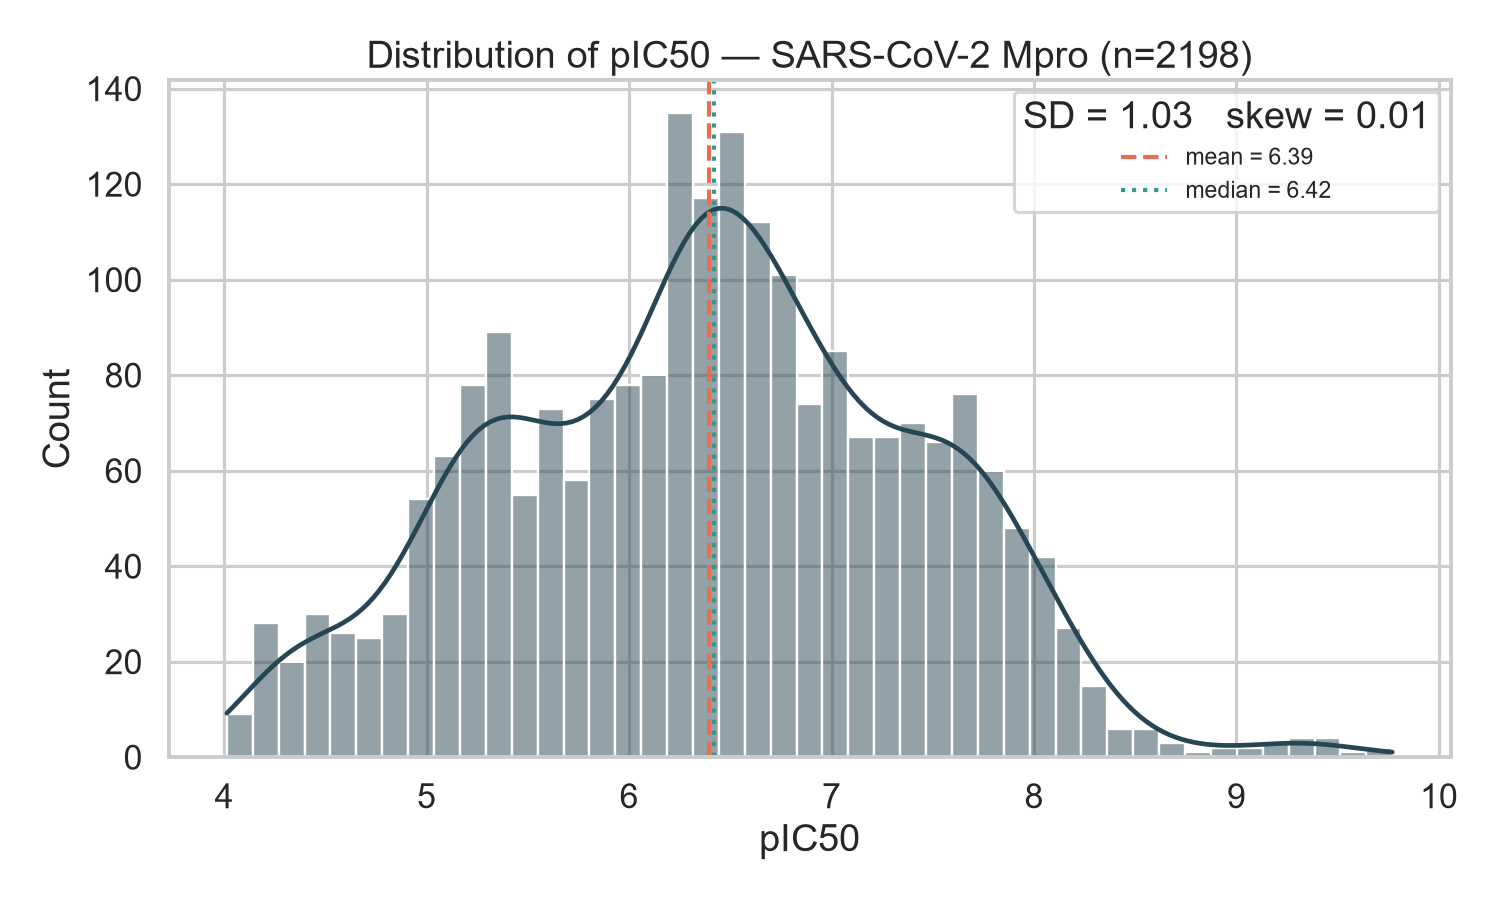
\includegraphics[width=0.86\textwidth]{../figures/fig01_pic50_distribution.png}
\caption{การแจกแจงความถี่ของค่า \pICfifty\ ในชุดข้อมูลหลัก}
\label{fig:pic50dist}
\end{figure}

\begin{figure}[H]
\centering
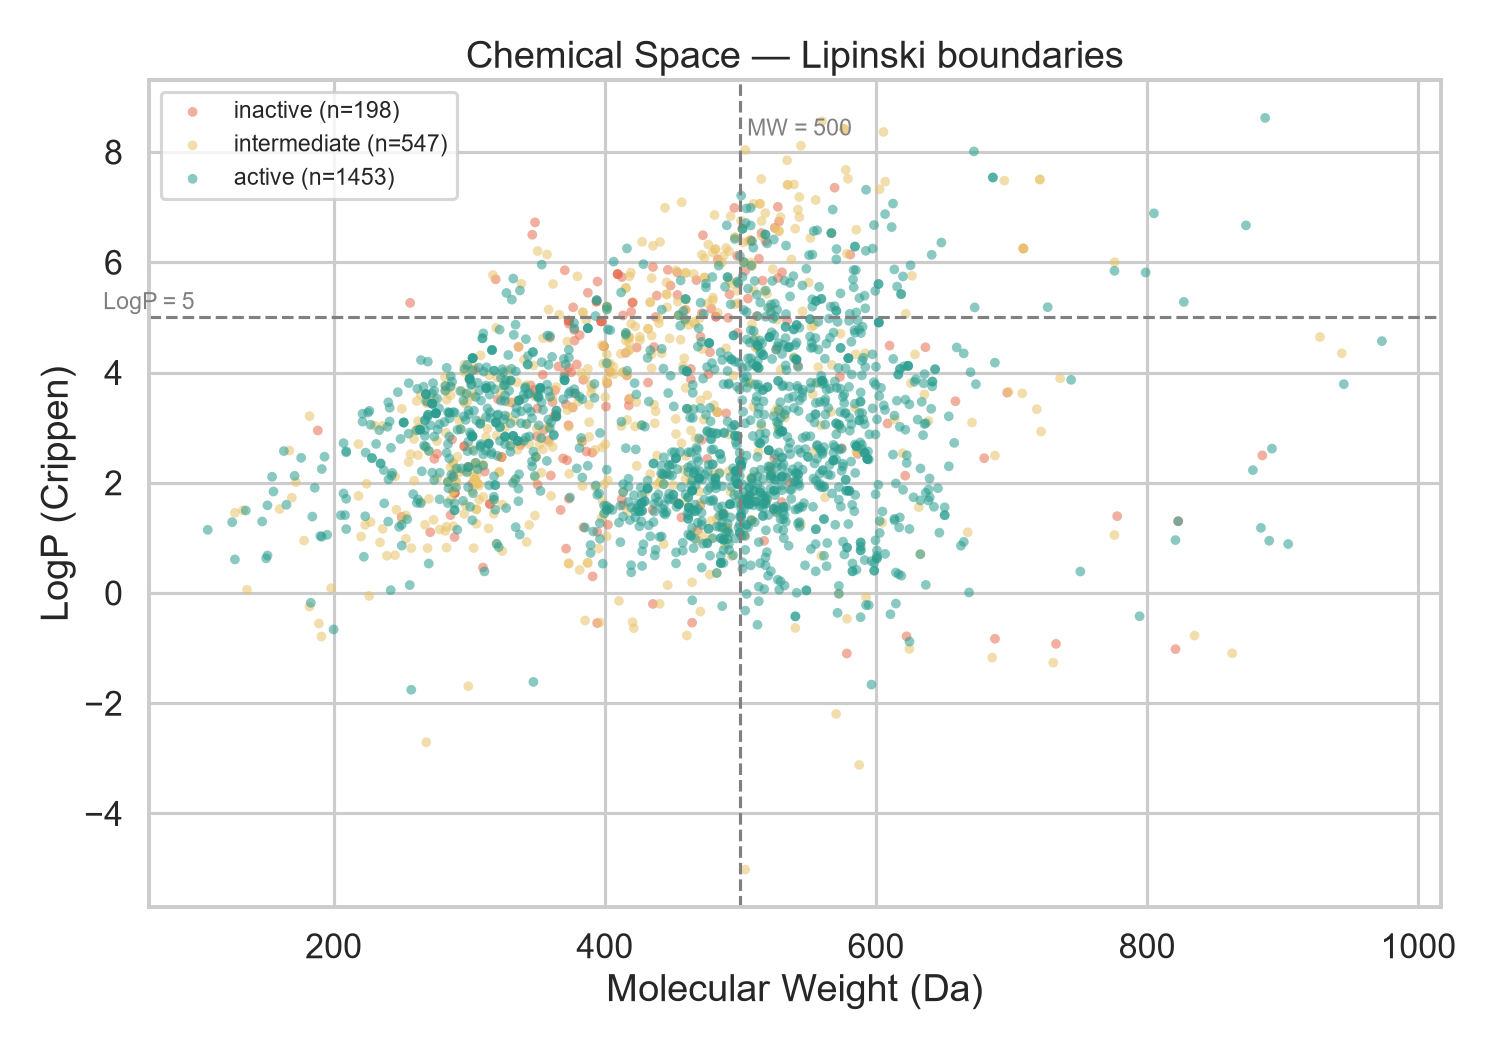
\includegraphics[width=0.82\textwidth]{../figures/fig02_chemical_space_mw_logp.png}
\caption{ปริภูมิเคมีระหว่างน้ำหนักโมเลกุลกับค่า LogP แยกตามกลุ่มฤทธิ์}
\label{fig:chemspace}
\end{figure}

\begin{figure}[H]
\centering
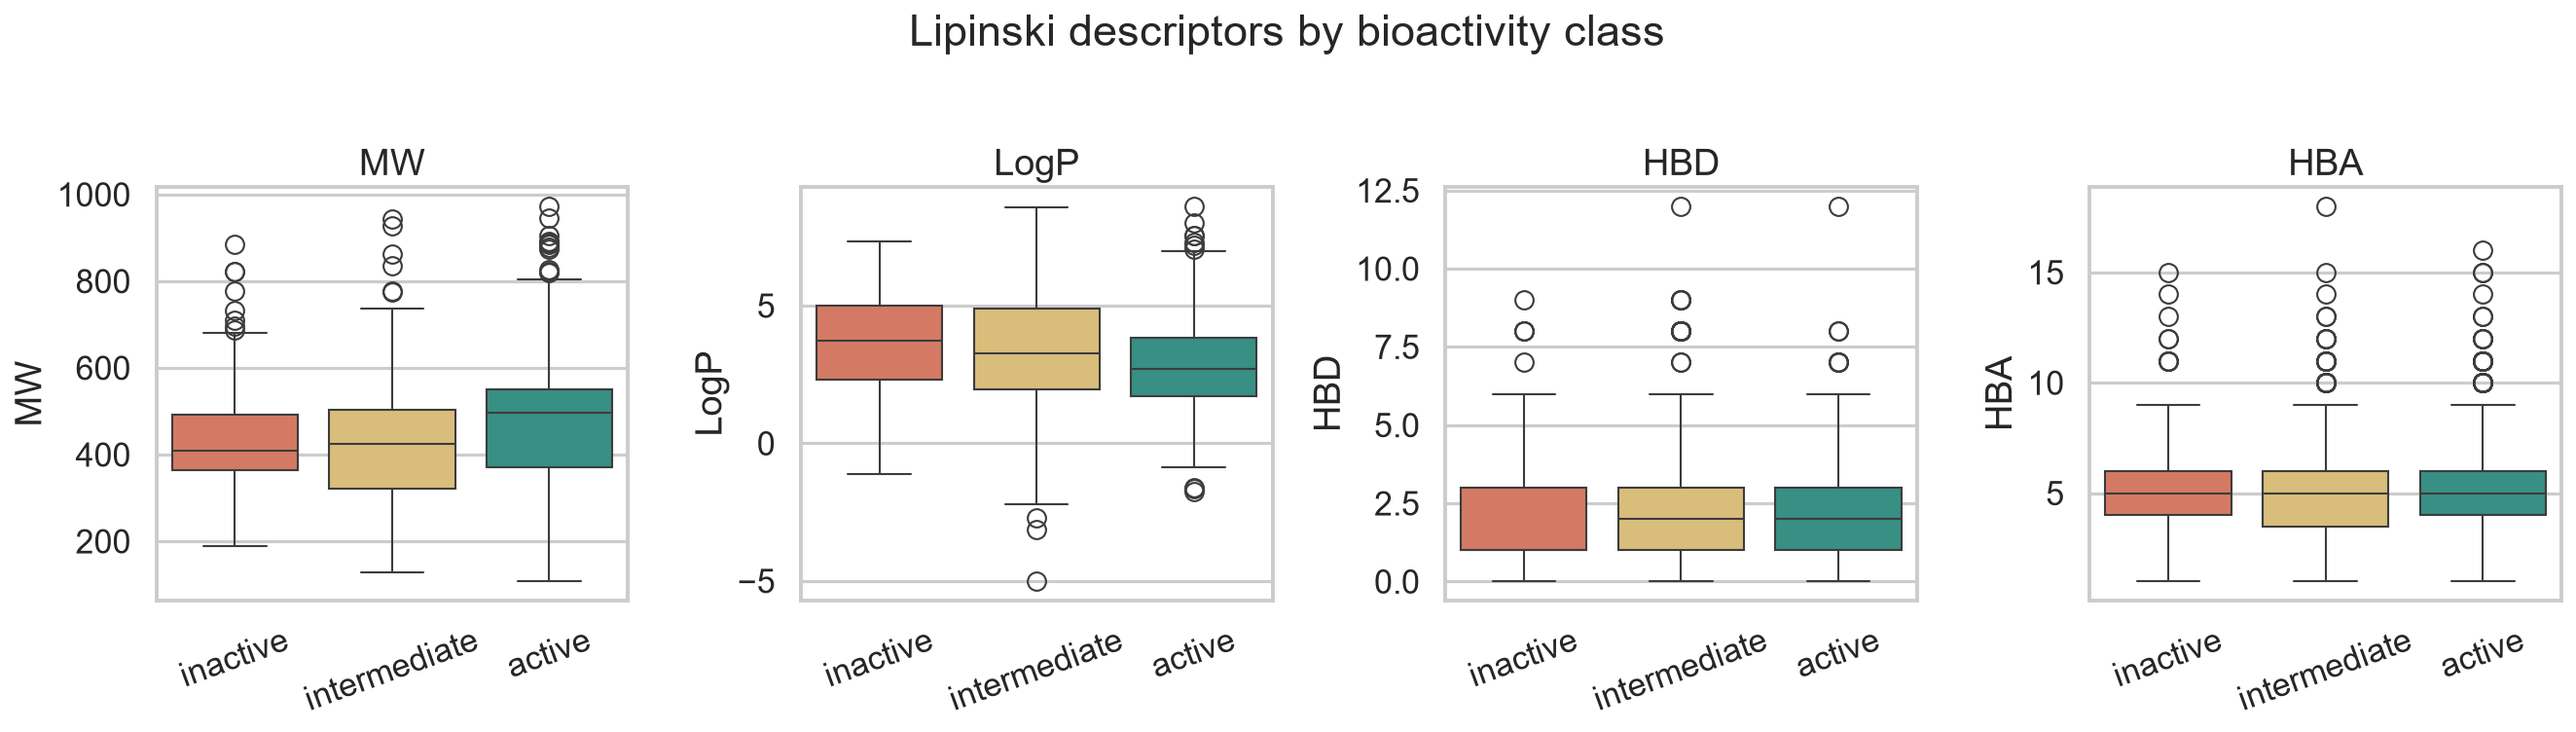
\includegraphics[width=\textwidth]{../figures/fig02b_lipinski_by_class.png}
\caption{การเปรียบเทียบ Lipinski Descriptors ตามกลุ่มฤทธิ์}
\label{fig:lipinskibox}
\end{figure}

\begin{figure}[H]
\centering
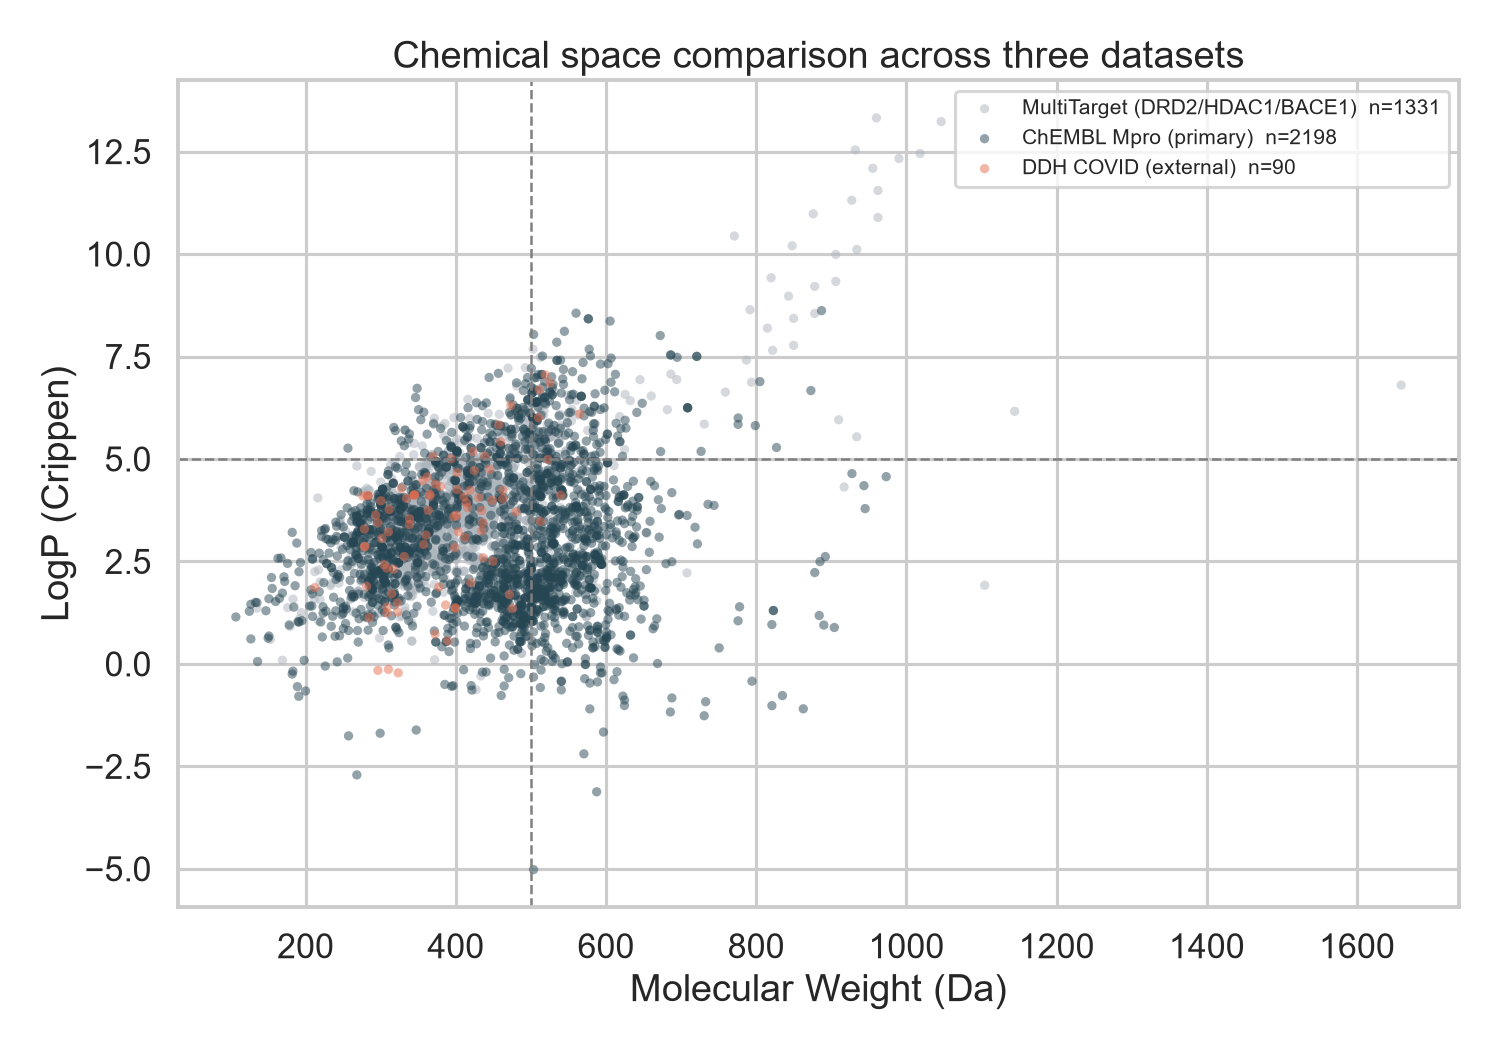
\includegraphics[width=0.82\textwidth]{../figures/fig02c_chemspace_3sets.png}
\caption{การเปรียบเทียบปริภูมิเคมีของชุดข้อมูลสามชุด}
\label{fig:chemspace3}
\end{figure}

\begin{table}[H]
\centering
\caption{โครงสร้างแกนกลาง Murcko 10 อันดับแรก}
\label{tab:scaffolds}
\small
\begin{tabular}{C{1.2cm} L{9.2cm} R{1.8cm} R{1.6cm}}
\toprule
\textbf{อันดับ} & \textbf{Murcko Scaffold} & \textbf{จำนวน} & \textbf{ร้อยละ}\\
\midrule
1 & \texttt{O=C(Oc1cccnc1)c1ccccc1} & 46 & 2.09\\
2 & \texttt{c1ccccc1} & 35 & 1.59\\
3 & \texttt{O=C(c1ccccc1)n1cnc2ccccc21} & 30 & 1.36\\
4 & \texttt{O=c1c2ccccc2[se]n1-c1ccccc1} & 29 & 1.32\\
5 & \texttt{O=c1[nH]c(-c2ccccc2)nc2ccccc12} & 27 & 1.23\\
6 & \texttt{O=C(Cn1sc2ccccc2c1=O)Nc1ccccc1} & 27 & 1.23\\
7 & \texttt{O=C(NCc1ccccc1)C(Nc1ccc(-c2ccccc2)cc1)c1cccnc1} & 27 & 1.23\\
8 & \texttt{O=C1NCCC1CCNC(=O)C1C2CC2CN1C(=O)c1cc2ccccc2[nH]1} & 25 & 1.14\\
9 & \texttt{O=C(NC(Cc1ccccc1)C(=O)NNCc1ccccc1)OCc1ccccc1} & 23 & 1.05\\
10 & \texttt{c1ccc(-c2cccc3c2CCc2c(-c4ccccn4)cccc2-3)cc1} & 22 & 1.00\\
\bottomrule
\end{tabular}
\end{table}

ไม่มี Scaffold ใดที่ครองสัดส่วนเกินร้อยละ 2.1 ซึ่งยืนยันความหลากหลายของชุดข้อมูลอีกครั้ง Scaffold อันดับ 8 มีลักษณะเป็นโครงสร้างเปปไทด์คล้าย ซึ่งสอดคล้องกับสารยับยั้ง \Mpro\ กลุ่มหลักที่พัฒนากันอยู่

\begin{table}[H]
\centering
\caption{การเปรียบเทียบ Lipinski Descriptors ด้วย Mann-Whitney U (active เทียบ inactive)}
\label{tab:mannwhitney}
\begin{tabular}{L{2.8cm} R{3.0cm} R{3.0cm} R{2.3cm} R{2.3cm}}
\toprule
\textbf{Descriptor} & \textbf{มัธยฐาน active} & \textbf{มัธยฐาน inactive} & \textbf{สถิติ U} & \textbf{ค่า p}\\
\midrule
MW & 496.39 & 409.49 & 177{,}509.5 & $8.85\times10^{-8}$\\
LogP & 2.710 & 3.725 & 106{,}106.5 & $2.01\times10^{-9}$\\
HBD & 2.00 & 1.00 & 165{,}977.5 & $3.38\times10^{-4}$\\
HBA & 5.00 & 5.00 & 160{,}018.5 & $8.86\times10^{-3}$\\
\bottomrule
\end{tabular}
\end{table}

ทุก descriptor แตกต่างกันอย่างมีนัยสำคัญทางสถิติที่ระดับ 0.01 โดยพบรูปแบบที่ชัดเจนคือ สารกลุ่ม active มี \textbf{น้ำหนักโมเลกุลสูงกว่า} (มัธยฐาน 496 เทียบกับ 409 Da) และ \textbf{ค่า LogP ต่ำกว่า} (2.71 เทียบกับ 3.73) สารกลุ่ม inactive อย่างมีนัยสำคัญ

รูปแบบนี้สอดคล้องกับความรู้ทางเคมียาที่ว่า สารยับยั้ง \Mpro\ ที่มีประสิทธิภาพมักเป็นโมเลกุลขนาดใหญ่ที่มีลักษณะคล้ายเปปไทด์ มีขั้วค่อนข้างสูง และมีหมู่ที่สร้างพันธะไฮโดรเจนกับกรดอะมิโนในช่องจับของเอนไซม์ได้ดี สังเกตได้จากค่า HBD ที่สูงกว่า อย่างไรก็ตาม น้ำหนักโมเลกุลมัธยฐานของสาร active ที่ 496 Da นั้นเกือบชนขีดจำกัดของกฎลิพินสกีที่ 500 Da ซึ่งสะท้อนความท้าทายในการพัฒนาสารกลุ่มนี้ให้เป็นยารับประทาน

\section{ผลการทำ Cross-Validation}

การแบ่งข้อมูลได้ผลดังนี้ Random Split ให้ชุดฝึก 1{,}648 โมเลกุลและชุดทดสอบ 550 โมเลกุล ส่วน Scaffold Split ให้ชุดฝึก 1{,}649 โมเลกุลและชุดทดสอบ 549 โมเลกุล

\begin{table}[H]
\centering
\caption{ผล 5-Fold Cross-Validation บนชุดฝึก Random Split (E1)}
\label{tab:cve1}
\small
\begin{tabular}{L{3.2cm} C{2.8cm} R{1.7cm} R{1.7cm} R{1.7cm} R{1.7cm}}
\toprule
\textbf{แบบจำลอง} & \textbf{CV \Rsq\ (เฉลี่ย $\pm$ SD)} & \textbf{RMSE} & \textbf{MAE} & \textbf{Train \Rsq} & \textbf{Gap}\\
\midrule
Dummy Regressor & $-0.0021 \pm 0.0013$ & 1.0371 & 0.8395 & 0.0000 & 0.0021\\
\textbf{Random Forest} & $\mathbf{0.5997 \pm 0.0394}$ & \textbf{0.6544} & 0.4481 & 0.9368 & 0.3371\\
XGBoost & $0.5803 \pm 0.0342$ & 0.6707 & 0.4531 & 0.9573 & 0.3770\\
SVR (RBF) & $0.5994 \pm 0.0461$ & 0.6549 & \textbf{0.4433} & 0.9703 & 0.3709\\
\bottomrule
\end{tabular}
\end{table}

\begin{table}[H]
\centering
\caption{ผล 5-Fold Cross-Validation บนชุดฝึก Scaffold Split (E2)}
\label{tab:cve2}
\small
\begin{tabular}{L{3.2cm} C{2.8cm} R{1.7cm} R{1.7cm} R{1.7cm} R{1.7cm}}
\toprule
\textbf{แบบจำลอง} & \textbf{CV \Rsq\ (เฉลี่ย $\pm$ SD)} & \textbf{RMSE} & \textbf{MAE} & \textbf{Train \Rsq} & \textbf{Gap}\\
\midrule
Dummy Regressor & $-0.0037 \pm 0.0019$ & 1.0204 & 0.8173 & 0.0000 & 0.0037\\
Random Forest & $0.6670 \pm 0.0181$ & 0.5876 & 0.3993 & 0.9407 & 0.2736\\
XGBoost & $0.6527 \pm 0.0127$ & 0.6002 & 0.4035 & 0.9515 & 0.2988\\
\textbf{SVR (RBF)} & $\mathbf{0.6735 \pm 0.0132}$ & \textbf{0.5820} & \textbf{0.3911} & 0.9609 & 0.2875\\
\bottomrule
\end{tabular}
\end{table}

ในระยะ Cross-Validation แบบจำลองทั้งสามที่ไม่ใช่ Dummy ให้ผลใกล้เคียงกันมาก โดย Random Forest นำเล็กน้อยในกรณี Random Split ค่า Dummy Regressor ที่ได้ \Rsq\ ติดลบเล็กน้อยเป็นไปตามที่คาดในทางทฤษฎี

ส่วนต่างระหว่าง Train \Rsq\ กับ CV \Rsq\ อยู่ในช่วง 0.27--0.38 ในทุกแบบจำลอง แสดงว่ามีการเรียนรู้เกินอยู่พอสมควร โดยเฉพาะ SVR ที่มี Train \Rsq\ สูงถึง 0.9703 ซึ่งเป็นลักษณะปกติของแบบจำลองที่ทำงานบนคุณลักษณะมิติสูง

\begin{table}[H]
\centering
\caption{ผลการศึกษา Ablation}
\label{tab:ablation}
\begin{tabular}{C{1.6cm} L{5.0cm} R{2.3cm} R{2.1cm} R{2.1cm}}
\toprule
\textbf{การทดลอง} & \textbf{คุณลักษณะ} & \textbf{จำนวนมิติ} & \textbf{CV \Rsq} & \textbf{CV RMSE}\\
\midrule
E4 & Lipinski เท่านั้น & 4 & 0.2668 & 0.8875\\
E3 & Morgan FP เท่านั้น & 1{,}024 & 0.5885 & 0.6636\\
\textbf{E1} & \textbf{Hybrid (FP + Lipinski)} & \textbf{1{,}028} & \textbf{0.5997} & \textbf{0.6544}\\
\bottomrule
\end{tabular}
\end{table}

ผลการศึกษา Ablation แสดงว่าคุณลักษณะแบบผสมให้ผลดีที่สุด โดยดีกว่าการใช้ Morgan FP อย่างเดียว $+0.0112$ \Rsq\ และดีกว่าการใช้ Lipinski อย่างเดียว $+0.3329$ \Rsq

\begin{keynote}
พลังการทำนายส่วนใหญ่มาจาก Morgan Fingerprints ขณะที่ Lipinski Descriptors เพิ่มค่าเพียงเล็กน้อย อย่างไรก็ตาม การเพิ่มขึ้น 0.0112 \Rsq\ จากการเพิ่มคุณลักษณะเพียง 4 มิติ คิดเป็นร้อยละ 0.39 ของจำนวนมิติทั้งหมด ถือว่าคุ้มค่าในเชิงอัตราส่วนต้นทุนต่อผลตอบแทน
\end{keynote}

\begin{table}[H]
\centering
\caption{ผลการพิสูจน์ Data Leakage}
\label{tab:leakage}
\begin{tabular}{C{1.6cm} L{7.2cm} R{2.3cm} R{2.3cm}}
\toprule
\textbf{การทดลอง} & \textbf{กรณี} & \textbf{CV \Rsq} & \textbf{ส่วนต่าง}\\
\midrule
E5 & A ถูกต้อง --- ปรับสเกลภายใน Pipeline & 0.5994 & ---\\
E5 & B ผิด --- ปรับสเกลก่อนแบ่งข้อมูล & 0.5995 & $\mathbf{+0.0001}$\\
\midrule
E5b & A ถูกต้อง --- SelectKBest ภายใน Pipeline & 0.5892 & ---\\
E5b & B ผิด --- SelectKBest บนข้อมูลทั้งชุด & 0.6008 & $\mathbf{+0.0116}$\\
\bottomrule
\end{tabular}
\end{table}

ผลการทดลองนี้เป็นข้อค้นพบที่ต้องรายงานอย่างตรงไปตรงมา เนื่องจากไม่เป็นไปตามที่คาดการณ์ไว้ล่วงหน้า

\textbf{การทดลอง E5 แสดงว่า Preprocessing Leakage แทบไม่มีผลเลย} ส่วนต่างเพียง $+0.0001$ \Rsq\ อธิบายได้จากสองเหตุผล ประการแรก มีเพียง 4 คุณลักษณะจากทั้งหมด 1{,}028 คุณลักษณะที่ผ่านการปรับสเกล คิดเป็นร้อยละ 0.39 เท่านั้น ประการที่สอง ขนาดชุดฝึก 1{,}648 ตัวอย่างมีขนาดใหญ่เพียงพอที่ค่าเฉลี่ยและส่วนเบี่ยงเบนมาตรฐานที่คำนวณจากชุดฝึกของแต่ละ Fold แทบไม่ต่างจากที่คำนวณจากข้อมูลทั้งชุด

\textbf{การทดลอง E5b แสดงว่า Feature Selection Leakage ให้อคติบวกที่วัดได้จริง} ส่วนต่าง $+0.0116$ \Rsq\ ซึ่งมากกว่า E5 ถึง 116 เท่า การรั่วไหลรูปแบบนี้ตรงกับสิ่งที่ตรวจพบในไฟล์ \texttt{xfinal.csv} ที่ได้รับมอบมา ซึ่งคัดเลือกคุณลักษณะ 300 ตัวจาก 4{,}262 คอลัมน์บนข้อมูลทั้งชุด ผลการทดลองนี้จึงเป็นหลักฐานเชิงประจักษ์ที่สนับสนุนการตัดสินใจไม่ใช้ไฟล์ดังกล่าว

\section{ผลการปรับจูนและประเมินบนชุดทดสอบ}

\begin{table}[H]
\centering
\caption{ไฮเปอร์พารามิเตอร์ที่ดีที่สุด (Random Split)}
\label{tab:bestparams}
\small
\begin{tabular}{L{3.0cm} L{10.6cm}}
\toprule
\textbf{แบบจำลอง} & \textbf{ค่าที่เลือกได้}\\
\midrule
Random Forest & \texttt{n\_estimators}=500, \texttt{max\_depth}=None, \texttt{min\_samples\_split}=5, \texttt{min\_samples\_leaf}=1, \texttt{max\_features}=0.3\\
XGBoost & \texttt{n\_estimators}=600, \texttt{learning\_rate}=0.03, \texttt{max\_depth}=8, \texttt{subsample}=0.8, \texttt{colsample\_bytree}=0.6\\
SVR (RBF) & \texttt{C}=1, \texttt{gamma}='scale', \texttt{epsilon}=0.05\\
\bottomrule
\end{tabular}
\end{table}

\begin{table}[H]
\centering
\caption{ผลการประเมินบนชุดทดสอบ Random Split ($n = 550$)}
\label{tab:testrandom}
\begin{tabular}{L{3.4cm} R{2.2cm} R{2.2cm} R{2.2cm} R{2.4cm}}
\toprule
\textbf{แบบจำลอง} & \textbf{\Rsq} & \textbf{RMSE} & \textbf{MAE} & \textbf{Spearman $\rho$}\\
\midrule
Dummy Regressor & $-0.0000$ & 1.0074 & 0.8054 & ---\\
Random Forest & 0.6822 & 0.5679 & 0.4107 & 0.8351\\
\textbf{XGBoost} & $\mathbf{0.7034}$ & $\mathbf{0.5487}$ & $\mathbf{0.3918}$ & $\mathbf{0.8415}$\\
SVR (RBF) & 0.6716 & 0.5774 & 0.4199 & 0.8257\\
\bottomrule
\end{tabular}
\end{table}

\begin{table}[H]
\centering
\caption{ผลการประเมินบนชุดทดสอบ Scaffold Split ($n = 549$)}
\label{tab:testscaffold}
\begin{tabular}{L{3.4cm} R{2.2cm} R{2.2cm} R{2.2cm} R{2.4cm}}
\toprule
\textbf{แบบจำลอง} & \textbf{\Rsq} & \textbf{RMSE} & \textbf{MAE} & \textbf{Spearman $\rho$}\\
\midrule
Dummy Regressor & $-0.0162$ & 1.0611 & 0.8715 & ---\\
Random Forest & 0.4949 & 0.7481 & 0.5626 & 0.7414\\
\textbf{XGBoost} & $\mathbf{0.5127}$ & $\mathbf{0.7348}$ & $\mathbf{0.5440}$ & $\mathbf{0.7452}$\\
SVR (RBF) & 0.4637 & 0.7708 & 0.5866 & 0.7057\\
\bottomrule
\end{tabular}
\end{table}

\textbf{XGBoost ให้ผลดีที่สุดบนชุดทดสอบทั้งสองวิธีการแบ่ง} ซึ่งน่าสนใจเพราะในระยะ Cross-Validation ก่อนปรับจูน XGBoost ทำได้ต่ำที่สุดในสามแบบจำลอง ผลนี้แสดงว่า XGBoost ได้ประโยชน์จากการปรับจูนไฮเปอร์พารามิเตอร์มากกว่าแบบจำลองอื่น โดยค่าที่เลือกได้คือ \texttt{learning\_rate} ต่ำที่ 0.03 ร่วมกับจำนวนต้นไม้มากที่ 600 ต้น ซึ่งเป็นการแลกความเร็วกับความแม่นยำ

\begin{keynote}[ประเด็นสำคัญที่สุดของบทนี้]
ค่า \Rsq\ ของ XGBoost ลดลงจาก 0.7034 บน Random Split เหลือ 0.5127 บน Scaffold Split คิดเป็นการลดลงร้อยละ 27.1 ส่วนต่างนี้ยืนยันคำเตือนของ Sheridan (2013) ว่าการแบ่งข้อมูลแบบสุ่มให้ค่าที่มองโลกในแง่ดีเกินไป เพราะโมเลกุลในอนุกรมเคมีเดียวกันกระจายอยู่ทั้งสองฝั่ง ในทางปฏิบัติ ตัวเลขที่ควรอ้างอิงเมื่อพูดถึงการทำนายสารที่มีโครงสร้างแกนกลางใหม่คือ $\Rsq = 0.5127$ ไม่ใช่ 0.7034
\end{keynote}

\begin{figure}[H]
\centering
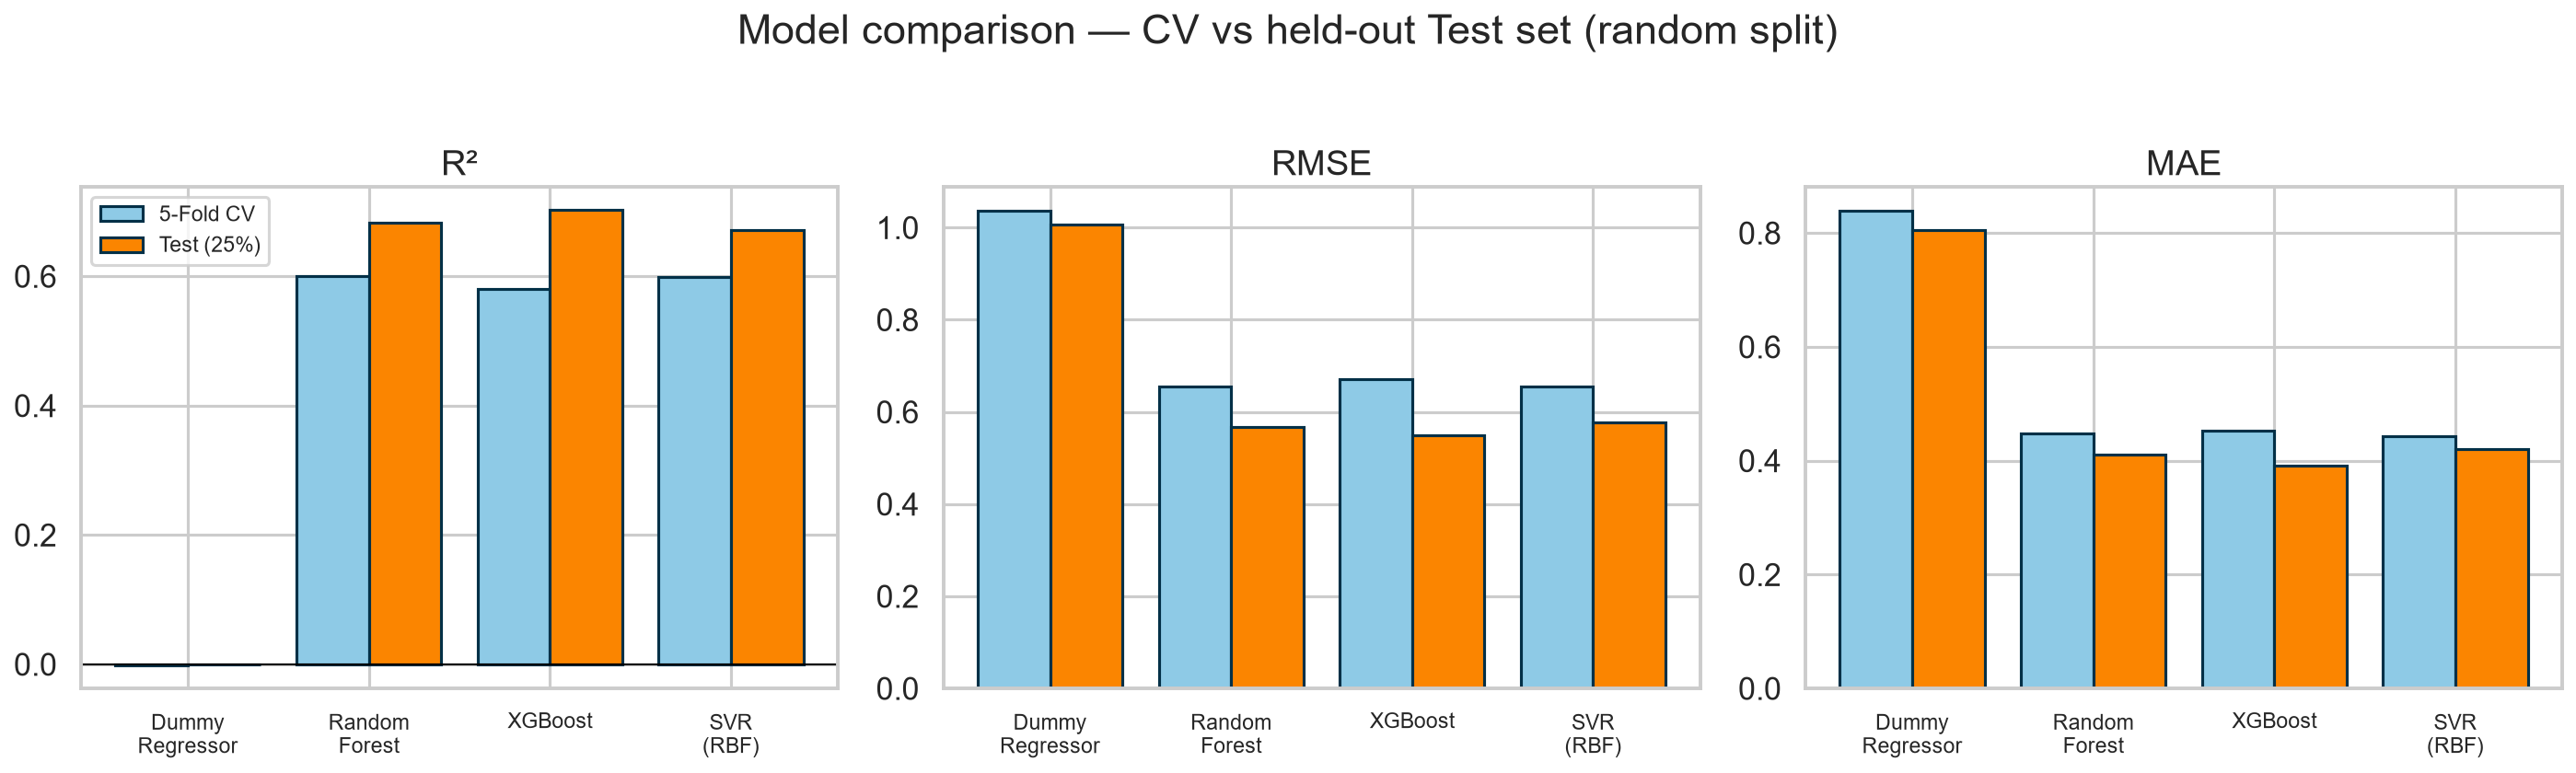
\includegraphics[width=\textwidth]{../figures/fig03_model_comparison.png}
\caption{การเปรียบเทียบประสิทธิภาพแบบจำลองระหว่าง Cross-Validation กับชุดทดสอบ}
\label{fig:modelcomp}
\end{figure}

\section{การวิเคราะห์ค่าคลาดเคลื่อน}

ค่าคลาดเคลื่อนโดยรวมของแบบจำลอง XGBoost บนชุดทดสอบ Random Split มีค่าเฉลี่ย $-0.0368$ และส่วนเบี่ยงเบนมาตรฐาน 0.5479 log unit การทำนายร้อยละ 93.6 มีความคลาดเคลื่อนไม่เกิน 1 log unit และร้อยละ 72.5 ไม่เกิน 0.5 log unit

\begin{figure}[H]
\centering
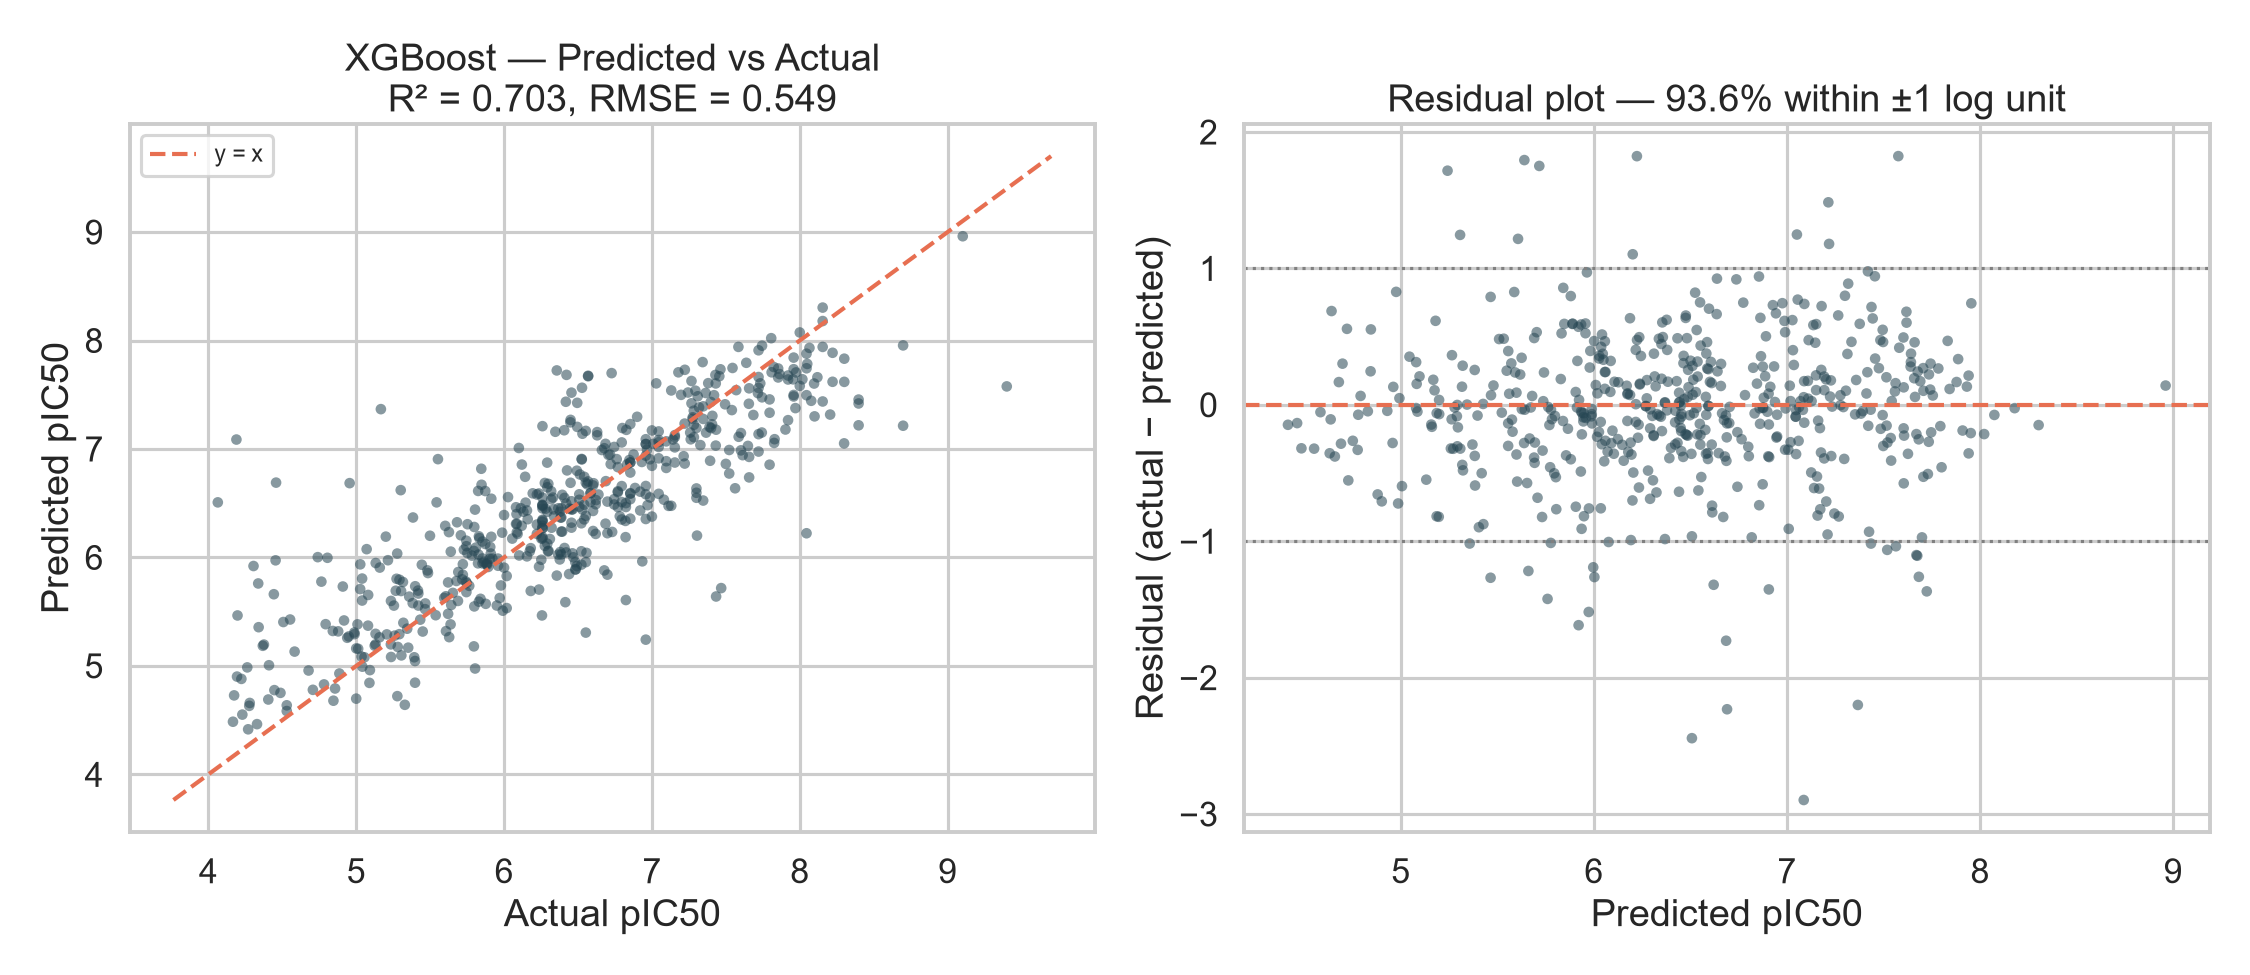
\includegraphics[width=\textwidth]{../figures/fig04_residual_plot.png}
\caption{กราฟค่าทำนายเทียบค่าจริง (ซ้าย) และกราฟค่าคลาดเคลื่อน (ขวา)}
\label{fig:residual}
\end{figure}

\begin{figure}[H]
\centering
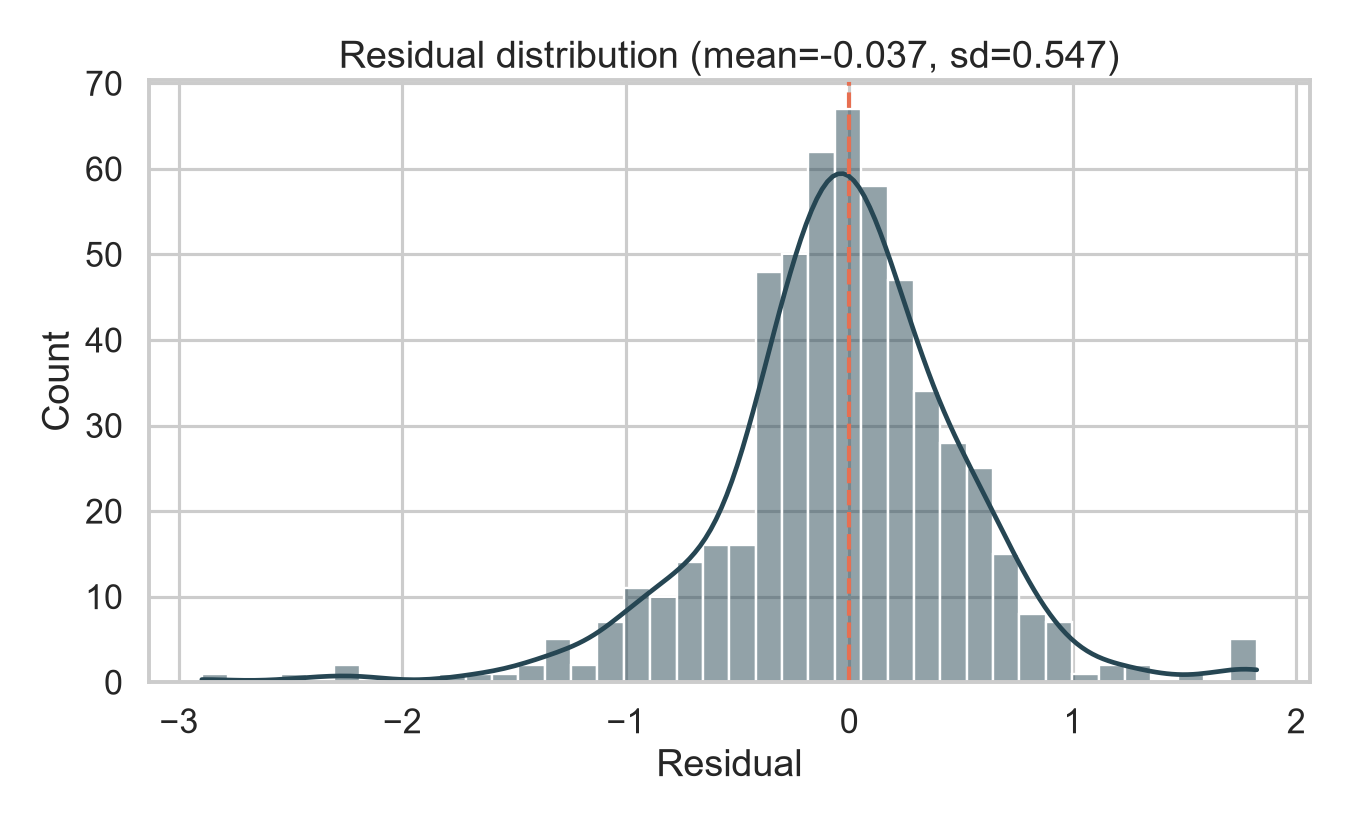
\includegraphics[width=0.76\textwidth]{../figures/fig04b_residual_hist.png}
\caption{การแจกแจงค่าคลาดเคลื่อน}
\label{fig:residualhist}
\end{figure}

\begin{table}[H]
\centering
\caption{การวิเคราะห์ค่าคลาดเคลื่อนแยกตามกลุ่มฤทธิ์}
\label{tab:residualclass}
\begin{tabular}{L{3.4cm} R{2.0cm} R{3.4cm} R{2.2cm} R{2.2cm}}
\toprule
\textbf{กลุ่มฤทธิ์} & \textbf{จำนวน} & \textbf{ค่าคลาดเคลื่อนเฉลี่ย} & \textbf{MAE} & \textbf{RMSE}\\
\midrule
active & 364 & $+0.1203$ & 0.3635 & 0.4926\\
intermediate & 137 & $-0.2116$ & 0.3481 & 0.4790\\
\textbf{inactive} & \textbf{49} & $\mathbf{-0.7151}$ & \textbf{0.7246} & \textbf{0.9667}\\
\bottomrule
\end{tabular}
\end{table}

ผลการวิเคราะห์นี้เปิดเผยจุดอ่อนสำคัญของแบบจำลอง กล่าวคือ \textbf{แบบจำลองทำนายสารกลุ่ม inactive สูงเกินจริงอย่างเป็นระบบเฉลี่ย 0.72 log unit} และมีค่า RMSE สูงถึง 0.9667 เกือบสองเท่าของอีกสองกลุ่ม

สาเหตุมาจากความไม่สมดุลของชุดข้อมูลฝึก ซึ่งมีสาร active ถึง 1{,}453 ตัว แต่มี inactive เพียง 198 ตัว คิดเป็นอัตราส่วน 7.3 ต่อ 1 แบบจำลองจึงมีแนวโน้มเอนเอียงไปทางการทำนายค่าสูง

ค่าคลาดเคลื่อนที่มากที่สุดสามอันดับแรกล้วนเป็นสารกลุ่ม inactive ที่ถูกทำนายเป็น active ได้แก่ ค่าจริง 4.190 ทำนาย 7.087 (คลาดเคลื่อน $-2.897$), ค่าจริง 4.064 ทำนาย 6.508 (คลาดเคลื่อน $-2.444$) และค่าจริง 4.458 ทำนาย 6.690 (คลาดเคลื่อน $-2.232$)

ข้อค้นพบนี้มีนัยสำคัญเชิงปฏิบัติ เพราะในงานคัดกรองยา การทำนายสารที่ไม่มีฤทธิ์ว่ามีฤทธิ์ (False Positive) จะทำให้เสียทรัพยากรไปกับการทดสอบสารที่ไม่มีประโยชน์

\section{ผลการวิเคราะห์ SHAP และ SAR}

แบบจำลองที่ใช้วิเคราะห์คือ XGBoost ซึ่งเป็นแบบจำลองประเภทต้นไม้ที่ให้ผลดีที่สุด คำนวณค่า SHAP บนชุดทดสอบ 400 โมเลกุล

\begin{table}[H]
\centering
\caption{ค่าความสำคัญของคุณลักษณะ 20 อันดับแรก}
\label{tab:shapimp}
\small
\begin{tabular}{C{1.4cm} L{2.6cm} R{2.6cm} L{4.6cm}}
\toprule
\textbf{อันดับ} & \textbf{คุณลักษณะ} & \textbf{Mean$|$SHAP$|$} & \textbf{ประเภท}\\
\midrule
1 & \textbf{MW} & \textbf{0.1165} & \textbf{Lipinski descriptor}\\
2 & FP\_10 & 0.0561 & Morgan fingerprint bit\\
3 & FP\_904 & 0.0557 & Morgan fingerprint bit\\
4 & FP\_301 & 0.0484 & Morgan fingerprint bit\\
5 & \textbf{HBA} & \textbf{0.0392} & \textbf{Lipinski descriptor}\\
6 & FP\_847 & 0.0365 & Morgan fingerprint bit\\
7 & FP\_578 & 0.0364 & Morgan fingerprint bit\\
8 & FP\_684 & 0.0361 & Morgan fingerprint bit\\
9 & FP\_807 & 0.0304 & Morgan fingerprint bit\\
10 & FP\_794 & 0.0303 & Morgan fingerprint bit\\
11 & \textbf{LogP} & \textbf{0.0288} & \textbf{Lipinski descriptor}\\
12 & FP\_583 & 0.0277 & Morgan fingerprint bit\\
13 & FP\_675 & 0.0242 & Morgan fingerprint bit\\
14 & FP\_759 & 0.0207 & Morgan fingerprint bit\\
15 & FP\_482 & 0.0196 & Morgan fingerprint bit\\
16 & \textbf{HBD} & \textbf{0.0196} & \textbf{Lipinski descriptor}\\
17 & FP\_206 & 0.0193 & Morgan fingerprint bit\\
18 & FP\_117 & 0.0184 & Morgan fingerprint bit\\
19 & FP\_330 & 0.0180 & Morgan fingerprint bit\\
20 & FP\_305 & 0.0172 & Morgan fingerprint bit\\
\bottomrule
\end{tabular}
\end{table}

\begin{keynote}[ข้อค้นพบที่สำคัญที่สุด]
น้ำหนักโมเลกุลเป็นคุณลักษณะที่มีอิทธิพลสูงสุด โดยมีค่า Mean$|$SHAP$|$ = 0.1165 ซึ่งสูงกว่าบิต Fingerprint ที่ดีที่สุดถึง 2.08 เท่า และ \textbf{Lipinski Descriptors ติดอันดับ 20 แรกครบทั้ง 4 ตัว}
\end{keynote}

ผลนี้ดูขัดแย้งกับผลการศึกษา Ablation ที่พบว่าการเพิ่ม Lipinski เข้าไปเพิ่มค่า \Rsq\ เพียง 0.0112 คำอธิบายคือ Morgan Fingerprints เข้ารหัสข้อมูลเกี่ยวกับขนาดและองค์ประกอบของโมเลกุลไว้โดยอ้อมอยู่แล้ว เพราะโมเลกุลใหญ่ย่อมมีบิตถูกเซ็ตมากกว่า เมื่อตัด Lipinski ออก แบบจำลองจึงสามารถชดเชยด้วยการรวมสารสนเทศจากบิตหลายบิตแทน คุณลักษณะ Lipinski จึง \textbf{สำคัญแต่ซ้ำซ้อน (Important but Redundant)} ซึ่งเป็นสถานการณ์ที่พบได้ทั่วไปเมื่อวิเคราะห์ความสำคัญของคุณลักษณะ

\begin{figure}[H]
\centering
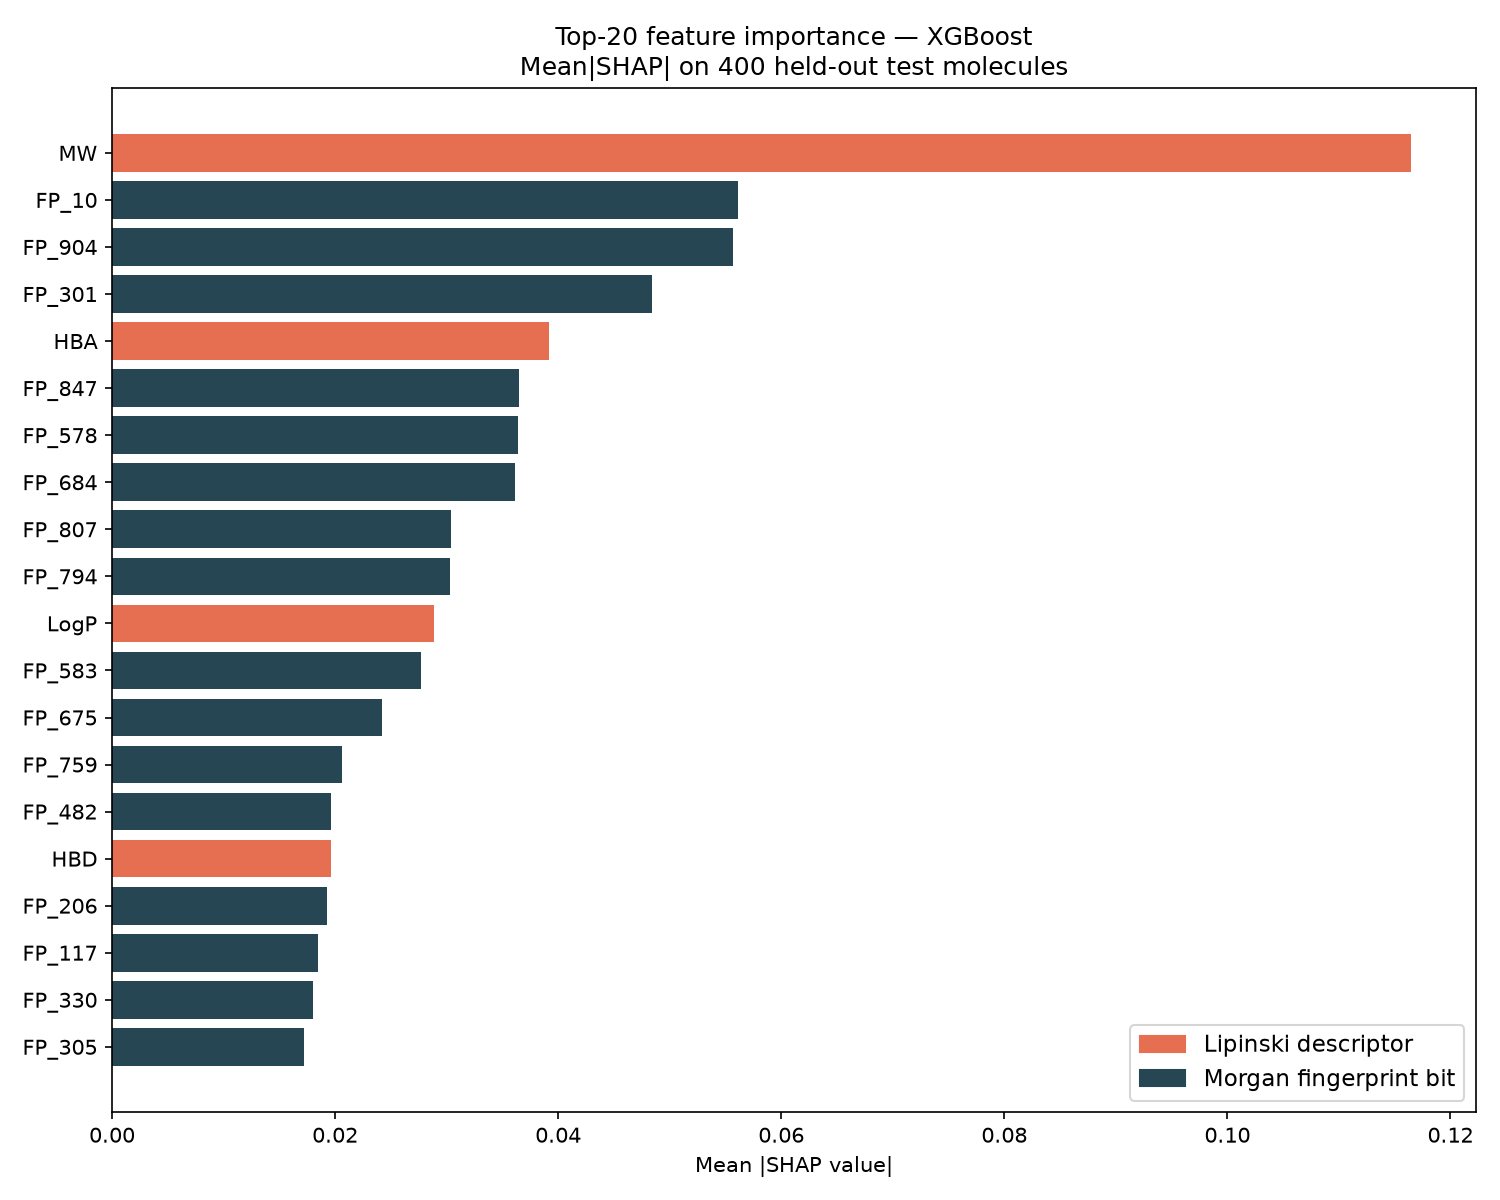
\includegraphics[width=0.80\textwidth]{../figures/fig05_shap_bar_top20.png}
\caption{ค่าความสำคัญของคุณลักษณะ 20 อันดับแรกโดย Mean$|$SHAP$|$}
\label{fig:shapbar}
\end{figure}

\begin{figure}[H]
\centering
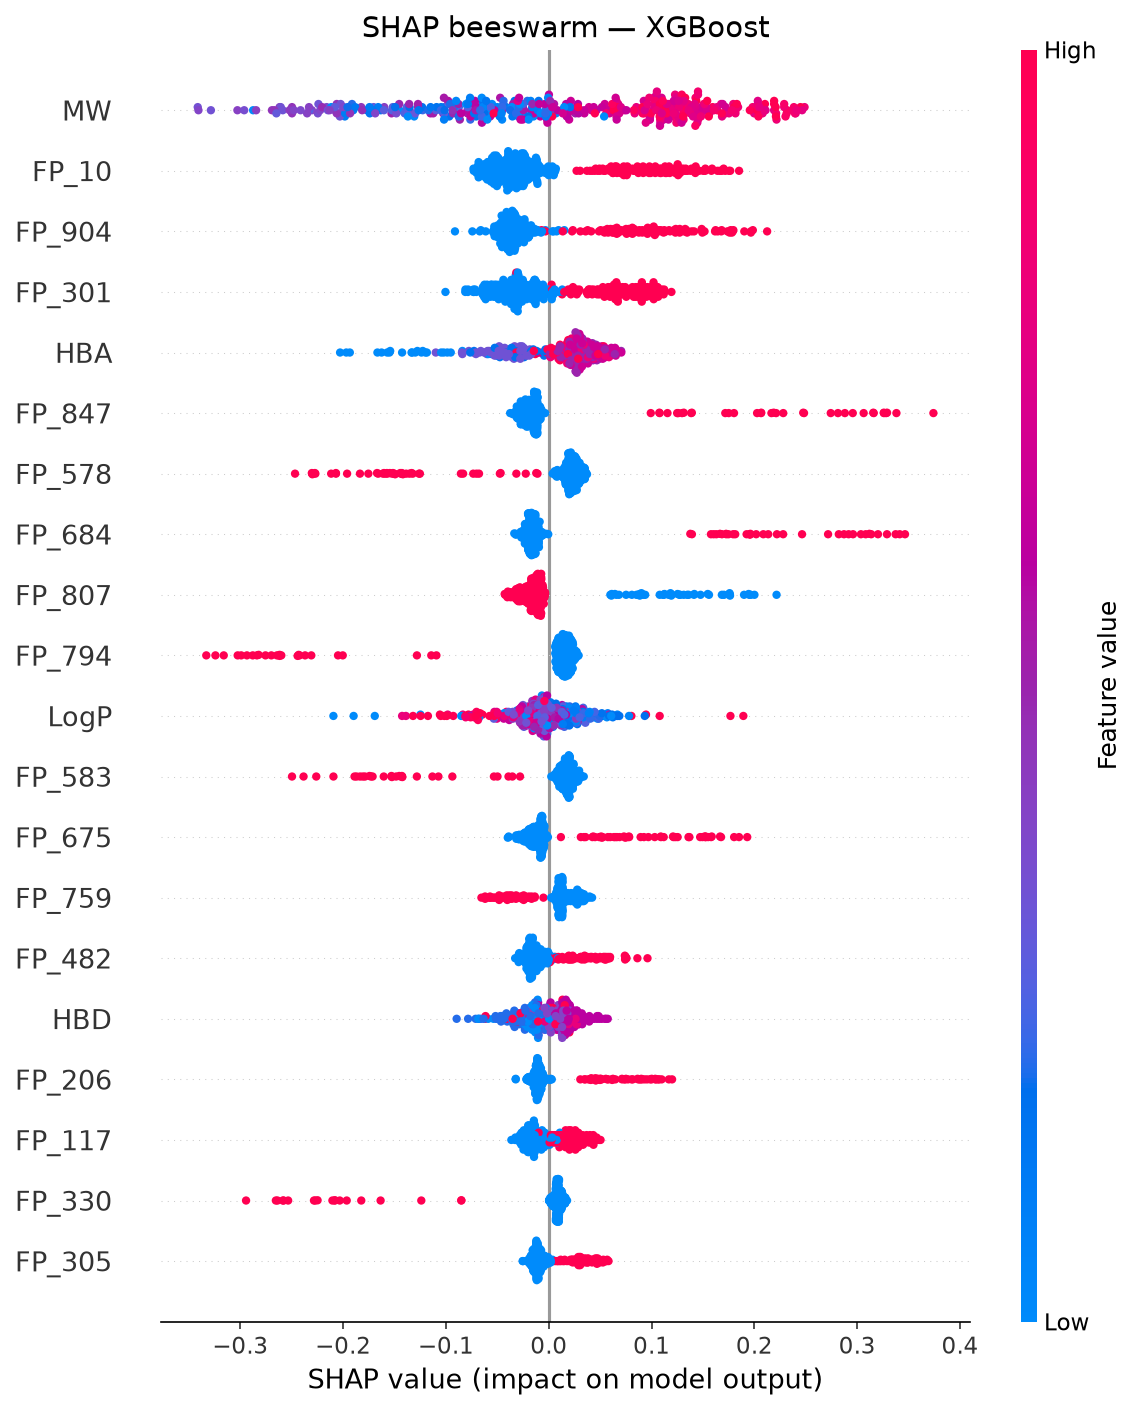
\includegraphics[width=0.80\textwidth]{../figures/fig06_shap_beeswarm.png}
\caption{SHAP Beeswarm Plot แสดงทิศทางอิทธิพลของแต่ละคุณลักษณะ}
\label{fig:beeswarm}
\end{figure}

\begin{figure}[H]
\centering
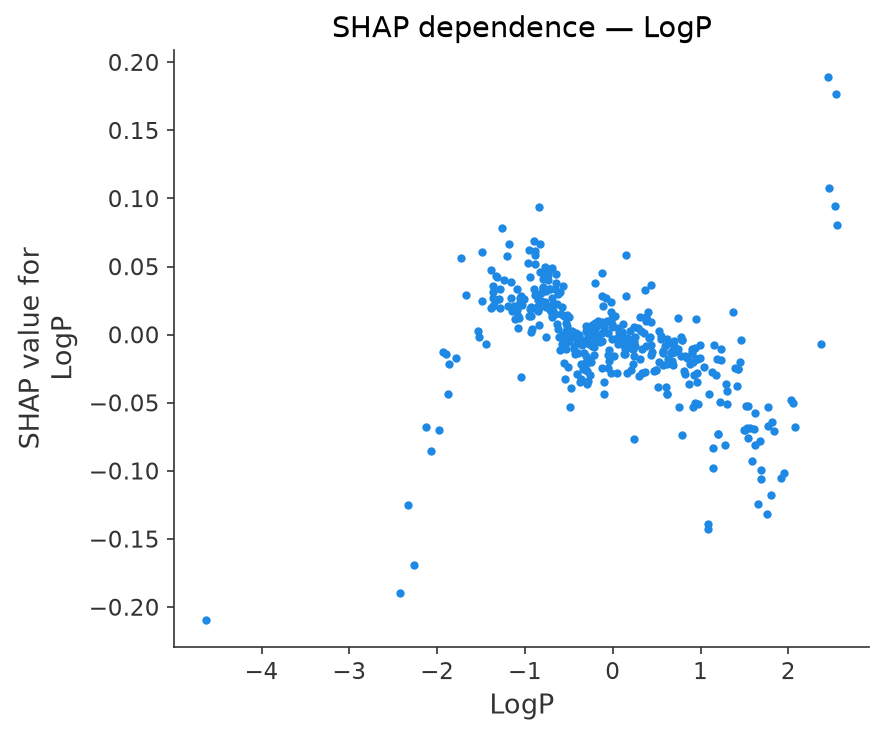
\includegraphics[width=0.72\textwidth]{../figures/fig06b_shap_dependence_logp.png}
\caption{SHAP Dependence Plot ของค่า LogP}
\label{fig:dependence}
\end{figure}

\begin{table}[H]
\centering
\caption{ตารางวิเคราะห์ SAR ของโครงสร้างย่อยที่สำคัญ}
\label{tab:sar}
\small
\begin{tabular}{L{1.8cm} R{1.8cm} L{2.0cm} R{2.0cm} R{1.6cm} R{1.8cm} R{1.6cm}}
\toprule
\textbf{บิต} & \shortstack{\textbf{Mean}\\\textbf{$|$SHAP$|$}} & \textbf{ทิศทาง} & \textbf{SHAP เมื่อบิต=1} & \textbf{\% ใน active} & \textbf{\% ใน inactive} & \textbf{จำนวน โมเลกุล}\\
\midrule
FP\_10 & 0.0561 & เพิ่มฤทธิ์ & $+0.1002$ & \textbf{41.9} & \textbf{4.5} & 696\\
FP\_904 & 0.0557 & เพิ่มฤทธิ์ & $+0.1005$ & 33.6 & 19.7 & 634\\
FP\_301 & 0.0484 & เพิ่มฤทธิ์ & $+0.0710$ & \textbf{50.9} & \textbf{13.1} & 908\\
FP\_578 & 0.0364 & ลดฤทธิ์ & $-0.1417$ & 6.1 & 25.8 & 276\\
FP\_807 & 0.0304 & ลดฤทธิ์ & $-0.0173$ & 84.4 & 95.5 & 1{,}904\\
FP\_794 & 0.0303 & ลดฤทธิ์ & $-0.2509$ & \textbf{2.0} & \textbf{19.7} & 130\\
\bottomrule
\end{tabular}
\end{table}

ผลการวิเคราะห์ SAR ให้ข้อมูลที่ตีความเชิงเคมีได้อย่างสอดคล้องกัน

\textbf{บิตที่เพิ่มฤทธิ์} บิต FP\_301 ปรากฏในสารกลุ่ม active ถึงร้อยละ 50.9 แต่ปรากฏในกลุ่ม inactive เพียงร้อยละ 13.1 คิดเป็นอัตราส่วนความเข้มข้น 3.9 เท่า และบิต FP\_10 มีอัตราส่วนสูงถึง 9.3 เท่า (ร้อยละ 41.9 เทียบกับ 4.5) โมเลกุลตัวอย่างที่มีบิต FP\_10 และมีค่า SHAP สูงสุดคือสารที่มีโครงสร้างเปปไทด์คล้ายพร้อมหมู่แอลดีไฮด์ที่ปลาย ซึ่งเป็นหมู่ที่ทราบกันดีว่าสร้างพันธะโควาเลนต์แบบผันกลับได้กับซิสเตอีนที่ตำแหน่ง 145 ในช่องเร่งปฏิกิริยาของ \Mpro

\textbf{บิตที่ลดฤทธิ์} บิต FP\_794 ปรากฏในกลุ่ม inactive ร้อยละ 19.7 แต่ปรากฏในกลุ่ม active เพียงร้อยละ 2.0 และมีค่า SHAP เฉลี่ยเมื่อบิตถูกเซ็ตติดลบมากที่สุดที่ $-0.2509$ โมเลกุลตัวอย่างเป็นสารกลุ่มพอลิไซคลิกอะโรมาติกที่ไม่มีหมู่ฟังก์ชันสำหรับสร้างพันธะโควาเลนต์

\begin{warnnote}[ข้อสังเกตเชิงระเบียบวิธี]
บิต FP\_807 มีลักษณะพิเศษคือปรากฏในโมเลกุลถึง 1{,}904 ตัวจาก 2{,}198 ตัว (ร้อยละ 86.6) และปรากฏในทั้งกลุ่ม active (ร้อยละ 84.4) และ inactive (ร้อยละ 95.5) ในสัดส่วนใกล้เคียงกัน บิตนี้จึงเป็นโครงสร้างย่อยทั่วไปที่พบได้ในสารเกือบทุกตัว ค่า SHAP ที่ติดลบเล็กน้อยจึงไม่ควรตีความว่าโครงสร้างนี้ลดฤทธิ์อย่างมีความหมายทางเคมี แต่เป็นผลจากการที่แบบจำลองใช้บิตนี้เป็นค่าอ้างอิงพื้นฐานมากกว่า
\end{warnnote}

\begin{figure}[H]
\centering
\begin{tabular}{ccc}
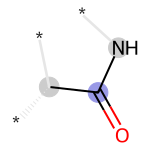
\includegraphics[width=0.24\textwidth]{../figures/fig07_bit_10_substructure.png} &
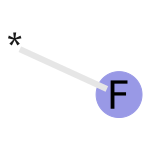
\includegraphics[width=0.24\textwidth]{../figures/fig07_bit_904_substructure.png} &
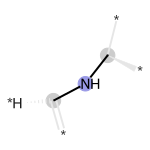
\includegraphics[width=0.24\textwidth]{../figures/fig07_bit_301_substructure.png}\\
(ก) บิต 10 --- เพิ่มฤทธิ์ & (ข) บิต 904 --- เพิ่มฤทธิ์ & (ค) บิต 301 --- เพิ่มฤทธิ์\\[1.2em]
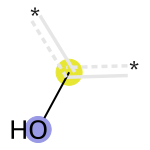
\includegraphics[width=0.24\textwidth]{../figures/fig07_bit_578_substructure.png} &
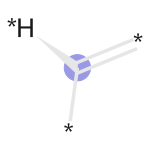
\includegraphics[width=0.24\textwidth]{../figures/fig07_bit_807_substructure.png} &
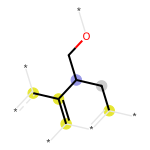
\includegraphics[width=0.24\textwidth]{../figures/fig07_bit_794_substructure.png}\\
(ง) บิต 578 --- ลดฤทธิ์ & (จ) บิต 807 --- ลดฤทธิ์ & (ฉ) บิต 794 --- ลดฤทธิ์\\
\end{tabular}
\caption{โครงสร้างย่อย 2 มิติของบิตสำคัญทั้ง 6 บิตที่ได้จากการจับคู่ย้อนกลับ}
\label{fig:bits}
\end{figure}

\section{ผลการทดสอบข้ามชุดข้อมูล}

\begin{table}[H]
\centering
\caption{ผลการทดสอบข้ามชุดข้อมูลกับ DDH COVID-19}
\label{tab:external}
\begin{tabular}{L{8.4cm} R{4.0cm}}
\toprule
\textbf{ตัวชี้วัด} & \textbf{ค่า}\\
\midrule
จำนวนสาร (หลังตัดที่ซ้ำกับชุดฝึก 4 ตัว) & 90\\
\textbf{\Rsq} & $\mathbf{-1.7191}$\\
RMSE & 1.3504\\
MAE & 1.2031\\
\textbf{Spearman $\rho$} & $\mathbf{0.5203}$\\
ค่าคลาดเคลื่อนเฉลี่ย (Bias) & $\mathbf{+1.1855}$\\
\bottomrule
\end{tabular}
\end{table}

\begin{warnnote}[ผลลบที่ต้องรายงานอย่างตรงไปตรงมา]
ค่า \Rsq\ ที่ติดลบหมายความว่าแบบจำลองทำนายชุด DDH ได้แย่กว่าการทายด้วยค่าเฉลี่ยของชุด DDH เอง และค่า Bias ที่ $+1.1855$ แสดงว่าแบบจำลองทำนายสูงเกินจริงอย่างเป็นระบบถึง 1.19 log unit หรือคิดเป็นการประเมินความแรงเกินจริงประมาณ 15 เท่า
\end{warnnote}

\begin{table}[H]
\centering
\caption{ผลการวิเคราะห์ Applicability Domain}
\label{tab:ad}
\begin{tabular}{L{5.2cm} R{1.7cm} R{2.4cm} R{1.9cm} R{2.1cm}}
\toprule
\textbf{ชุดข้อมูล} & \textbf{จำนวน} & \textbf{Tanimoto เฉลี่ย} & \textbf{มัธยฐาน} & \textbf{\% $< 0.4$}\\
\midrule
ChEMBL test (ในโดเมน) & 550 & 0.7541 & 0.7972 & \textbf{7.6}\\
DDH external & 90 & 0.3340 & 0.2897 & \textbf{84.4}\\
MultiTarget (นอกโดเมน) & 1{,}331 & 0.2880 & 0.2738 & \textbf{95.6}\\
\bottomrule
\end{tabular}
\end{table}

การวิเคราะห์ Applicability Domain อธิบายความล้มเหลวข้างต้นได้อย่างชัดเจน สารในชุด DDH ถึงร้อยละ 84.4 มีค่าความคล้ายคลึง Tanimoto สูงสุดต่อชุดฝึกต่ำกว่าเกณฑ์ 0.4 โดยมีค่ามัธยฐานเพียง 0.2897 ขณะที่ชุดทดสอบภายในมีเพียงร้อยละ 7.6 ที่อยู่นอกเกณฑ์ และมีค่ามัธยฐานสูงถึง 0.7972

กล่าวอีกนัยหนึ่ง ชุด DDH แทบเป็นสารคนละปริภูมิเคมีกับข้อมูลที่ใช้ฝึก โดยมีระดับความแตกต่างใกล้เคียงกับชุด MultiTarget ซึ่งเป็นสารที่ออกฤทธิ์ต่อเป้าหมายคนละชนิดโดยสิ้นเชิง (DRD2, HDAC1, BACE1)

นอกจากนี้ยังมีปัจจัยเสริมคือการเลื่อนของการกระจายตัวแปรตาม (Label Distribution Shift) โดยชุด ChEMBL มี \pICfifty\ เฉลี่ย 6.393 และประกอบด้วยสาร active เป็นส่วนใหญ่ ขณะที่ชุด DDH มีค่าเฉลี่ยเพียง 4.872 และเป็นสาร inactive ถึง 61 จาก 90 ตัว เมื่อประกอบกับจุดอ่อนของแบบจำลองที่ทำนายสาร inactive สูงเกินจริง จึงส่งผลให้ความคลาดเคลื่อนสะสมรุนแรงขึ้น

\begin{keynote}[สิ่งที่ยังใช้ได้]
ค่า Spearman $\rho$ = 0.5203 บ่งชี้ว่าแบบจำลองยังคงจัดอันดับสารได้ในระดับปานกลาง แม้ค่าสัมบูรณ์จะคลาดเคลื่อนมาก ในทางปฏิบัติหมายความว่าแบบจำลองยังพอใช้เป็นเครื่องมือจัดลำดับความสำคัญเพื่อคัดกรองเบื้องต้นได้ แต่ไม่ควรใช้ค่า \pICfifty\ ที่ทำนายได้เป็นตัวเลขสัมบูรณ์กับสารนอกโดเมน
\end{keynote}

\begin{figure}[H]
\centering
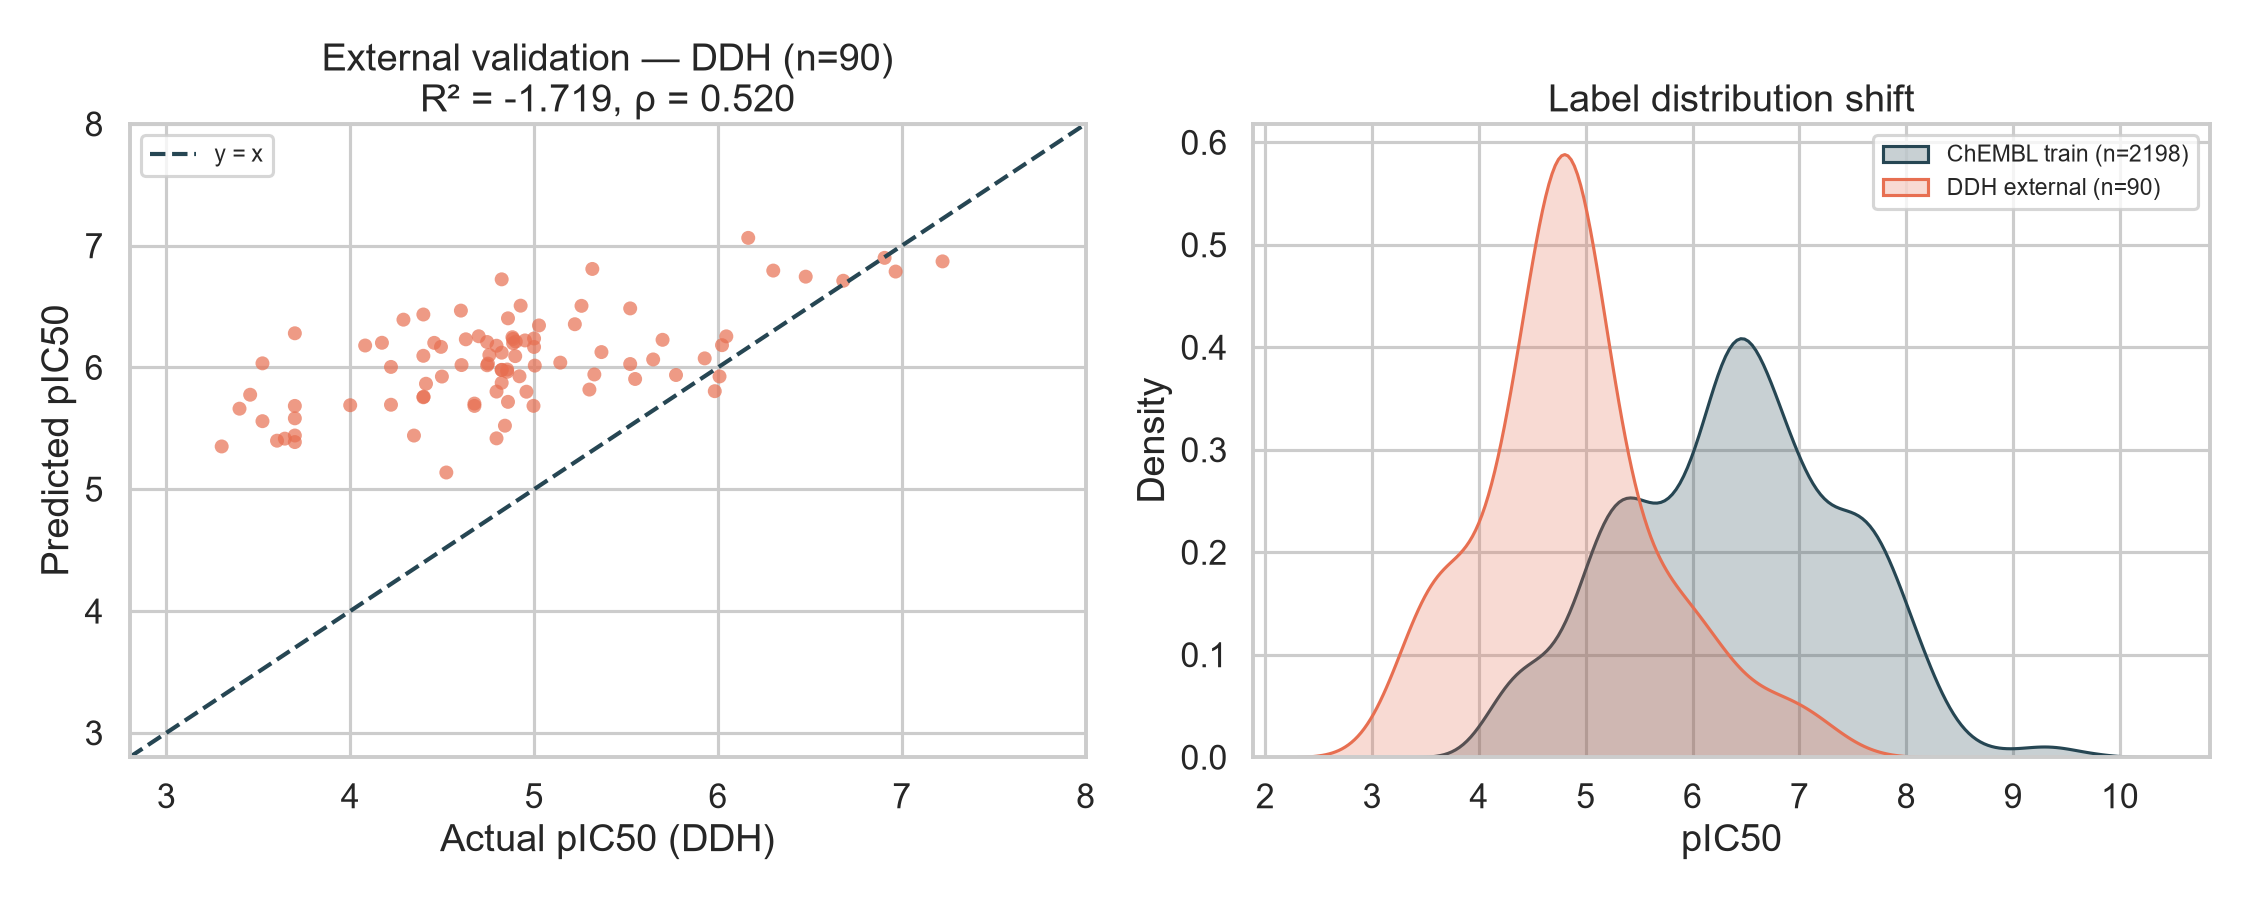
\includegraphics[width=\textwidth]{../figures/fig08_external_validation.png}
\caption{ผลการทดสอบข้ามชุดข้อมูล (ซ้าย) และการเลื่อนของการกระจายตัวแปรตาม (ขวา)}
\label{fig:extval}
\end{figure}

\begin{figure}[H]
\centering
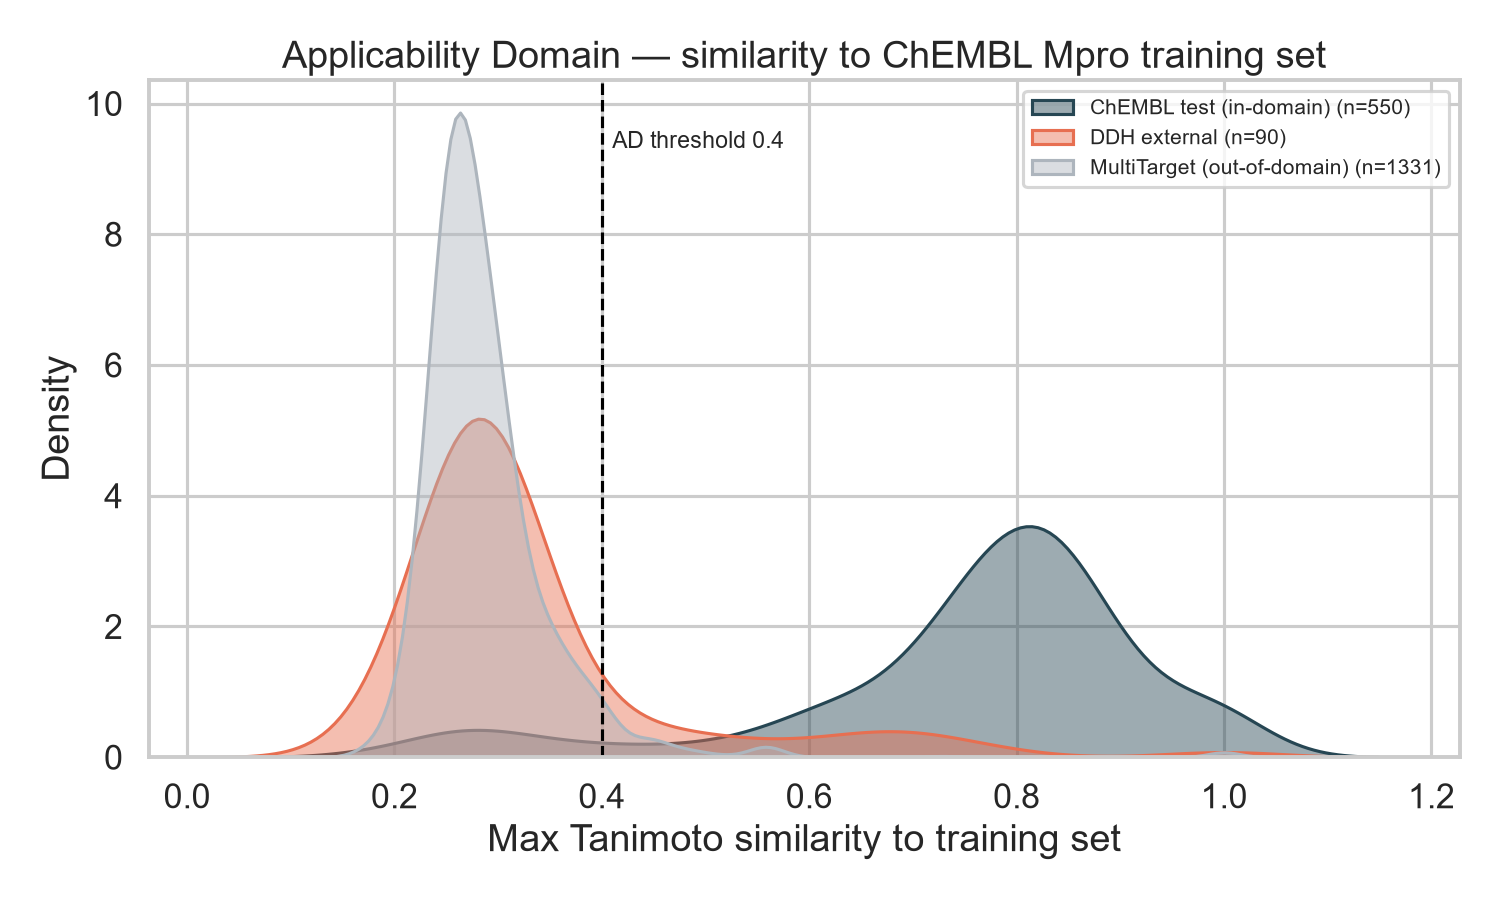
\includegraphics[width=0.82\textwidth]{../figures/fig09_applicability_domain.png}
\caption{การวิเคราะห์ Applicability Domain ด้วยค่าความคล้ายคลึง Tanimoto}
\label{fig:adfig}
\end{figure}

\begin{table}[H]
\centering
\caption{ผลการทำนายสาร BLINDED จำนวน 10 ตัว}
\label{tab:blinded}
\begin{tabular}{C{3.0cm} R{4.0cm} R{4.4cm}}
\toprule
\textbf{ลำดับสาร} & \textbf{\pICfifty\ ที่ทำนาย} & \textbf{\ICfifty\ ที่ทำนาย ($\mu$M)}\\
\midrule
4 & 5.476 & 3.345\\
23 & 5.833 & 1.469\\
28 & 5.810 & 1.549\\
42 & 5.994 & 1.014\\
46 & 6.225 & 0.596\\
58 & 6.546 & 0.285\\
\textbf{63} & \textbf{6.990} & \textbf{0.102}\\
68 & 6.500 & 0.316\\
74 & 6.251 & 0.561\\
95 & 5.868 & 1.355\\
\bottomrule
\end{tabular}
\end{table}

สารลำดับที่ 63 ได้รับการทำนายว่ามีฤทธิ์แรงที่สุด อย่างไรก็ตาม เนื่องจากสารกลุ่มนี้อยู่ในชุด DDH ซึ่งพบว่าอยู่นอก Applicability Domain เป็นส่วนใหญ่ ค่าทำนายเหล่านี้จึงควรถือเป็นเพียงการสาธิตการใช้งานระบบ และควรตีความในเชิงลำดับมากกว่าค่าสัมบูรณ์
